\documentclass[../../main.tex]{subfiles}
\begin{document}

{\bf [解]}
$f(x)=x^3+3x^2$ とすると一階，2階微分は
\begin{align}
f'(x) &=3x^2+6x = 3x(x+2) \label{eq:1}\\
f''(x)&=6x+6 = 6(x+1) 
\end{align}
だから増減表は以下のようになる．

\begin{table}[htb]
\centering
\caption{$f(x) = x^3 + 3x^2$ の増減表}
\begin{tabular}{c|ccccccccc}
$x$ & $\dots$ & $-2$ & $\dots$ & $-1$ & $\dots$ & $0$ & $\dots$ \\ \hline
$f'(x)$ & $+$ & $0$ & $-$ & $-$ & $-$ & $0$ & $+$ \\
$f''(x)$ & $-$ & $-$ & $-$ & $0$ & $+$ & $+$ & $+$ \\ \hline
$f(x)$ & $\text{\raisebox{-2pt}{$\curvearrowright$}}$ & $4$ & $\text{\raisebox{-2pt}{$\curvearrowleft$}}$ & $2$ & $\text{\raisebox{-2pt}{$\hookleftarrow$}}$ & $0$ & $\text{\raisebox{-2pt}{$\hookrightarrow$}}$ \\
 & & (極大) & & (変曲点) & & (極小) & 
\end{tabular}
\end{table}

従って$y=f(x)$の概形は以下のようになる．

\begin{figure}[htb]
\centering
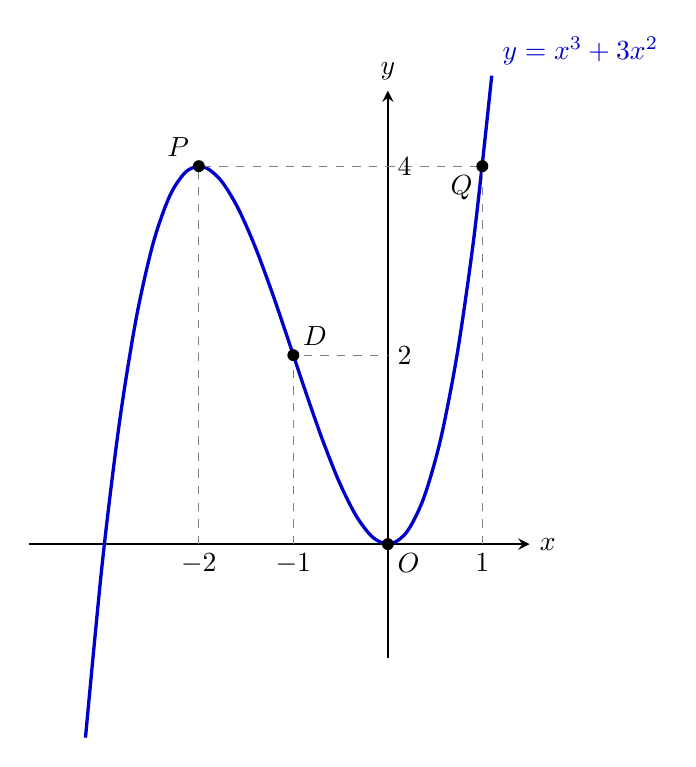
\begin{tikzpicture}[scale=1.2, >=stealth]
  % 1. 座標軸
  \draw[->, thick] (-3.8, 0) -- (1.5, 0) node[right] {$x$};
  \draw[->, thick] (0, -1.2) -- (0, 4.8) node[above] {$y$};
  
  % 原点 O
  \node[below right] at (0,0) {$\text{O}$};

  % 2. 曲線 y = x^3 + 3x^2
  \draw[domain=-3.2:1.1, smooth, very thick, blue!80!black] 
    plot (\x, {\x*\x*\x + 3*\x*\x}) node[above right] {$y = x^3 + 3x^2$};

  % 3. ガイド線（点線）
  % 極大点 P(-2, 4) からの点線
  \draw[dashed, gray] (-2, 0) -- (-2, 4) -- (0, 4);
  % Q(1, 4) からの点線
  \draw[dashed, gray] (1, 0) -- (1, 4) -- (0, 4);
  % 変曲点 D(-1, 2) からの点線
  \draw[dashed, gray] (-1, 0) -- (-1, 2) -- (0, 2);

  % 4. 各点とそのラベルのプロット
  % Q(1, 4) :
  \fill[black] (1, 4) circle (1.8pt) node[below left] {$\text{Q}$};
  
  % P(-2, 4) : 極大点
  \fill[black] (-2, 4) circle (1.8pt) node[above left] {$\text{P}$};
  
  % D(-1, 2) : 変曲点
  \fill[black] (-1, 2) circle (1.8pt) node[above right] {$\text{D}$};
  
  % O(0, 0) : 極小点・原点
  \fill[black] (0, 0) circle (1.8pt);

  % 軸上の目盛りラベル
  \node[below] at (-2, 0) {$-2$};
  \node[below] at (-1, 0) {$-1$};
  \node[below] at (1, 0) {$1$};
  \node[right] at (0, 4) {$4$};
  \node[right] at (0, 2) {$2$};

\end{tikzpicture}
\caption{$y = x^3 + 3x^2$ のグラフと主要な点 $O, P, Q, D$}
\end{figure}

次にR, Sを動かして良い領域について考える．
グラフの凹凸より，点RはDの中で自由に動かしても良いが点Sは場所によっては線分OSが領域Dの外に出る可能性がある．
そのために原点Oから$y=f(x)$に引いた接線について考えよう．

\cref{eq:1}より$x=t$ での接線は
\begin{align}
y=(3t^2+6t)x-2t^3-3t^2 \label{eq:2}
\end{align}
となる．これが$O$を通る時，
\begin{align}
2t^3+3t^2=0 \iff t=0,\ -\dfrac{3}{2}
\end{align}
であることに注意すると，非自明な解は$t=-\dfrac{3}{2}$である．この時の接線は\cref{eq:2}より
\begin{align}
 y = -\dfrac{9}{4}x \label{eq:3}
\end{align}
である．よって$\triangle ORS$が$D$に含まれるようなR,Sの可動領域は下図斜線部（境界含む）である．
ここで\cref{eq:3}と$y=4$の交点を$T\left(\dfrac{-16}{9},4\right)$とおいた．

\begin{figure}[htb]
\begin{center}
\begin{tikzpicture}[scale=1.1, >=stealth, every node/.style={font=\small}]

  % 1. 領域 E の斜線塗りつぶし
   \fill[pattern=north east lines, pattern color=black!50] plot[domain=1:-1.5,samples=60] (\x,{\x*\x*\x+3*\x*\x}) -- (-16/9,4) -- (1,4) -- cycle;

  % 2. 補助線（x軸への垂線・座標線）
  % S(-16/9, 4) からの垂線
  \draw[dashed, gray!70] (-16/9, 0) -- (-16/9, 4);
  % P(-2, 4) からの垂線
  \draw[dashed, gray!70] (-2, 0) -- (-2, 4);
  % Q(1, 4) からの垂線
  \draw[dashed, gray!70] (1, 0) -- (1, 4);
  % t = -3/2 の接点からの補助線 (x軸・y軸)
  \draw[dashed, gray!70] (-1.5, 0) -- (-1.5, 3.375) -- (0, 3.375);
  % y = 4 の水平補助線
  \draw[dashed, gray!70] (-2.3, 4) -- (0, 4);

  % 3. 座標軸描画
  \draw[->, thick] (-2.8, 0) -- (2.0, 0) node[right] {$x$};
  \draw[->, thick] (0, -0.8) -- (0, 5.5) node[above] {$y$};

  % 4. 曲線と直線
  % 曲線 y = x^3 + 3x^2
  \draw[domain=-2.55:1.15, smooth, thick, blue!80!black] plot (\x, {\x*\x*\x + 3*\x*\x});

  % 5. 点 R, S の座標定義と ORS の描画
  % E 領域内の適当な点 R, S を設定 (例: R = (-1.1, 3.2), S = (0.5, 3.5))
  \coordinate (O) at (0,0);
  \coordinate (R) at (-1.1, 3.2);
  \coordinate (S) at (0.7, 3.5);

  % △ORS の組み立て（赤枠線で強調）
  \draw[very thick, green!80!black] (O) -- (R) -- (S) -- cycle;
  \fill[green!10, opacity=0.5] (O) -- (R) -- (S) -- cycle; % ほんのり三角形内を塗りつぶし
  \fill (-1.1,3.2) circle (1.2pt) node[above] {$R$};
  \fill (0.7,3.5) circle (1.2pt) node[above] {$S$};


  
  % 水平線段 PQ
  \draw[thick] (-2, 4) -- (1, 4);
  
  % 接線 (S から接点を通り左上へ抜ける直線)
  \draw[thick, red!80!black] (-16/9, 4) -- (-1.5, 3.375);
  \draw[dashed, red!80!black] (-16/9, 4) -- (-2.3, 5.23); % 延長線
  \draw[dashed, red!80!black] (-16/9, 4) -- (0, 0); % 延長線

  % 5. 軸上の目盛りテキスト
  \node[below left] at (0,0) {$O$};
  \node[above left,font=\small] at (-2, 0) {$-2$};
  \node[below,font=\small] at (-16/9, 0) {$\frac{-16}{9}$};
  \node[above right,font=\small] at (-1.5, 0) {$\frac{-3}{2}$};
  \node[below] at (1, 0) {$1$};
  \node[above right] at (0, 4) {$4$};
  \node[right, font=\footnotesize] at (0, 3.375) {$\frac{27}{8}$};

  % 6. プロット点とラベル
  \fill (0,0) circle (1.2pt);
  \fill (-2,4) circle (1.2pt) node[above left] {$P$};
  \fill (1,4) circle (1.2pt) node[above right] {$Q$};
  \fill (-16/9,4) circle (1.2pt) node[above] {$T$};
  \fill[red!80!black] (-1.5, 3.375) circle (1.2pt);

  % 領域 E の名札
  \node[fill=white, inner sep=1pt, font=\bfseries] at (-0.6, 2.3) {$E$};

\end{tikzpicture}
\end{center}
\caption{R,Sが動ける範囲 $E$（斜線部）}
\end{figure}

さて，この時$\triangle ORS$の面積最大値を与える$R,S$の候補を考える．
まず$S$を固定して$R$を動かす．OSを底辺とみなすと，Rが領域Eの内部にある時，RからOSにおろした垂線上でRをさらに動かして領域Eの境界まで持って行くことで$\triangle ORS$の高さはより大きくなり，従って面積も大きくなる．よって$\triangle ORS$の面積が最大の時Rは領域Eの境界上にある．
全く同様に考えるとSも領域Eの境界上にある．従って，以下この場合のみ考えよう．

点Sは第二章限にあるから，その座標を$(s, ks)\, (k < 0)$とおく．この時線分OSと点Rの距離$\ell_1$は$R(x_1,y_1)$として
\begin{align}
 \ell_1=\dfrac{|kx_1+y_1|}{\sqrt{k^2+1}}=\dfrac{-kx_1+y_1}{\sqrt{k^2+1}} \quad (\because\ x_1,y_1\ge0,\ -k\ge0) \label{eq:4}
\end{align}
と書ける．$k<0$よりこれは$x_1,y_1$について単調増加だから，$\triangle ORS$の面積が最大になるのは $R(1,4)$ の時である．
この時線分ORの方程式は$y=4x$と書ける．

次にSを動かすことを考えると，$S$と$OR$の距離を最大にする$S$をもとめれば良い．$S(x_2,y_2)$としてこの距離を$\ell_2$とすると，
\begin{align}
\ell_2=\dfrac{|4x_2-y_2|}{\sqrt{17}}=\dfrac{-4x_2+y_2}{\sqrt{17}} \quad (\because\ x_2<0,\ y_2>0)
\end{align}
となる．これは$x_2$について単調減少，$y_2$について単調増加だから，最大値を与える$S$は$S\left(-\dfrac{16}{9},4\right)$である．

以上から，$S\left(-\dfrac{16}{9},4\right)$，$R(1,4)$の時に$\triangle ORS$の面積は最大で，その値は
\begin{align}
\dfrac{1}{2}\left|1\cdot4+\dfrac{16}{9}\cdot4\right|=\dfrac{50}{9}
\end{align}
となる．


\newpage

\end{document}
